% A LaTeX (non-official) template for ISAE projects reports
% Copyright (C) 2014 Damien Roque

% This program is free software; you can redistribute it and/or
% modify it under the terms of the GNU General Public License
% as published by the Free Software Foundation; either version 2
% of the License, or (at your option) any later version.

% This program is distributed in the hope that it will be useful,
% but WITHOUT ANY WARRANTY; without even the implied warranty of
% MERCHANTABILITY or FITNESS FOR A PARTICULAR PURPOSE.  See the
% GNU General Public License for more details.

% You should have received a copy of the GNU General Public License
% along with this program; if not, write to the Free Software
% Foundation, Inc., 51 Franklin Street, Fifth Floor, Boston, MA  02110-1301, USA.

% Version: 0.2
% Author: Damien Roque <damien.roque_AT_isae.fr>

\documentclass{beamer}
\usepackage[utf8]{inputenc}
\usepackage[english]{babel}
\usepackage{palatino}
\usepackage{graphicx}
\graphicspath{{./images/}}
\usepackage{colortbl}
\usepackage{xcolor}
\usepackage{tikz}
\usetikzlibrary{shapes,arrows}
\usetikzlibrary{mindmap,trees}
\usetikzlibrary{calc}
\usepackage{pgfplots}
\pgfplotsset{compat=newest}
\pgfplotsset{plot coordinates/math parser=false}
\newlength\figureheight
\newlength\figurewidth
\usepackage{ifthen}
\usepackage{subfigure}
\usepackage{amsthm}
\usepackage{amsfonts}
\usepackage{amssymb}
\usepackage{amsmath}
\usepackage{eurosym}
\usepackage{wasysym}
\usepackage{movie15}
\usepackage{float}
\usepackage{subfig}
\usepackage{bibentry}

% Printing on 2 slides per page
%\pgfpagesuselayout{2 on 1}[a4paper,border shrink=5mm]

% My macros...
\newcommand*{\SET}[1]  {\ensuremath{\boldsymbol{#1}}}
\newcommand*{\VEC}[1]  {\ensuremath{\boldsymbol{#1}}}
\newcommand*{\MAT}[1]  {\ensuremath{\boldsymbol{#1}}}
\newcommand*{\OP}[1]  {\ensuremath{\text{#1}}}
\newcommand*{\NORM}[1]  {\ensuremath{\left\|#1\right\|}}
\newcommand*{\DPR}[2]  {\ensuremath{\left \langle #1,#2 \right \rangle}}
\newcommand*{\calbf}[1]  {\ensuremath{\boldsymbol{\mathcal{#1}}}}
\newcommand*{\shift}[1]  {\ensuremath{\boldsymbol{#1}}}
\newcommand{\eqdef}{\stackrel{\mathrm{def}}{=}}
\newcommand{\argmax}{\operatornamewithlimits{argmax}}
\newcommand{\argmin}{\operatornamewithlimits{argmin}}
\newcommand{\ud}{\, \text{d}}
\newcommand{\vect}{\text{Vect}}
\newcommand{\sinc}{\text{sinc}}
\newcommand{\esp}{\ensuremath{\mathbb{E}}}
\newcommand{\hilbert}{\ensuremath{\mathcal{H}}}
\newcommand{\fourier}{\ensuremath{\mathcal{F}}}
\newcommand{\sgn}{\text{sgn}}
\newcommand{\intTT}{\int_{-T}^{T}}
\newcommand{\intT}{\int_{-\frac{T}{2}}^{\frac{T}{2}}}
\newcommand{\intinf}{\int_{-\infty}^{+\infty}}
\newcommand{\Sh}{\ensuremath{\boldsymbol{S}}}
\newcommand{\Cpx}{\ensuremath{\mathbb{C}}}
\newcommand{\R}{\ensuremath{\mathbb{R}}}
\newcommand{\Z}{\ensuremath{\mathbb{Z}}}
\newcommand{\N}{\ensuremath{\mathbb{N}}}
\newcommand{\K}{\ensuremath{\mathbb{K}}}
\newcommand{\reel}{\mathcal{R}}
\newcommand{\imag}{\mathcal{I}}
\newcommand{\cmnr}{c_{m,n}^\reel}
\newcommand{\cmni}{c_{m,n}^\imag}
\newcommand{\cnr}{c_{n}^\reel}
\newcommand{\cni}{c_{n}^\imag}
\newcommand{\LR}{\mathcal{L}_2(\R)}
\newcommand{\tproto}{g}
\newcommand{\rproto}{\check{g}}
\newcommand{\Tproto}{G}
\newcommand{\Rproto}{\check{G}}

%\theoremstyle{definition}
%\newtheorem{definition}{Définition}[subsection]

\theoremstyle{remark}
\newtheorem{remarque}{Remarque}[subsection]

\theoremstyle{plain}
\newtheorem{propriete}{Propriété}[subsection]
\newtheorem{exemple}{Exemple}[subsection]

% Choosing a main theme and a color theme
\mode<presentation> {
  %\usetheme{Warsaw}
  \usetheme{Madrid}
  %\usetheme{Frankfurt}
  \usecolortheme{seahorse}
}


\addtobeamertemplate{frametitle}{}{%
\vskip-1em
\begin{tikzpicture}[remember picture,overlay]
\node[anchor=north east,yshift=4pt] at (current page.north east) {
\includegraphics[height=0.8cm]{images/logo-isae-long-sans-texte}};
\end{tikzpicture}}

\title[Multitask and Transfer review]{Deep RL literature review on multitask and transfer}

\author[A. Quintela]{\small \textbf{Andrés Quintela \inst{1}}\\ Supervisor: Emmanuel Rachelson\inst{2}}

%\date{23 janvier 2014}

\institute[ISAE/DISC]
{
\vspace{0.5cm}
\begin{minipage}{0.7\linewidth}
  \begin{center}
    \inst{1} ISAE Supaero, Erasmus student from Imperial College London\\
    \vspace{0.2cm}
    \inst{2} ISAE Supaero, DISC, Supaero Reinforcement Learning (SuReLi)\\
    \vspace{1em}
    
\includegraphics[height=2.5cm]{images/logo-isae-long}
  \end{center}
\end{minipage}
}

% Clear the navigation bar
\setbeamertemplate{navigation symbols}{}
 
\subject{Multitask and transfer}

\begin{document}

\begin{frame}
\titlepage
\end{frame}

\begin{frame}
  \frametitle{Index}
  \small
  \tableofcontents
  \normalsize
\end{frame}

% Recall the outline at each section
\AtBeginSection[]
{%
\begin{frame}
  \frametitle{Index}
  \small
  %\tableofcontents[hideothersubsections]
  %\tableofcontents[currentsubsection,hideothersubsections]
  \tableofcontents[currentsection]
  \normalsize
\end{frame}
}

\section{Reinforcement learning}
\label{sec:RL}

\begin{frame}
  \frametitle{Reinforcement Learning (RL)}
\begin{itemize}


\item Markov Decision Process (MDP) :
  \begin{equation}
    \label{eq:tranformee-fourier}
    \langle S_{t}, A_{t}, R_{t}, S_{t+1} \rangle 
  \end{equation}

\item Policy $ \pi(a|s)  $. Learning $\xrightarrow{}$ finding the optimal policy

\item Objective: maximizing accumulated reward

\item Evaluation of how good it is to be in a given state and to take a certain action.
\begin{equation}
    q_{\pi}(s)=\mathop{\mathbb{E}}_{\pi} \Big [ \sum_{k=0}^{\infty} \gamma^k R_{t+k+1}\big | S_{t}=s ,A_{t}=a \Big ]
\end{equation}

\item Optimal policy chooses the action with the highest q-value.
\end{itemize}  

\end{frame}

\begin{frame}
  \frametitle{Deep RL}
\begin{itemize}
     
\item Algorithm $\xrightarrow{}$ estimate q-value function $\xrightarrow{}$ optimal policy \\
\item High-dimensional state and action spaces $\xrightarrow{}$ Can't explore the entire state-action space ( $\mathcal{S} \times \mathcal{A}$ )
\item Neural networks as q-value function approximators
\end{itemize}


\begin{figure}[!ht]
     \subfloat[Gridworld]{%
       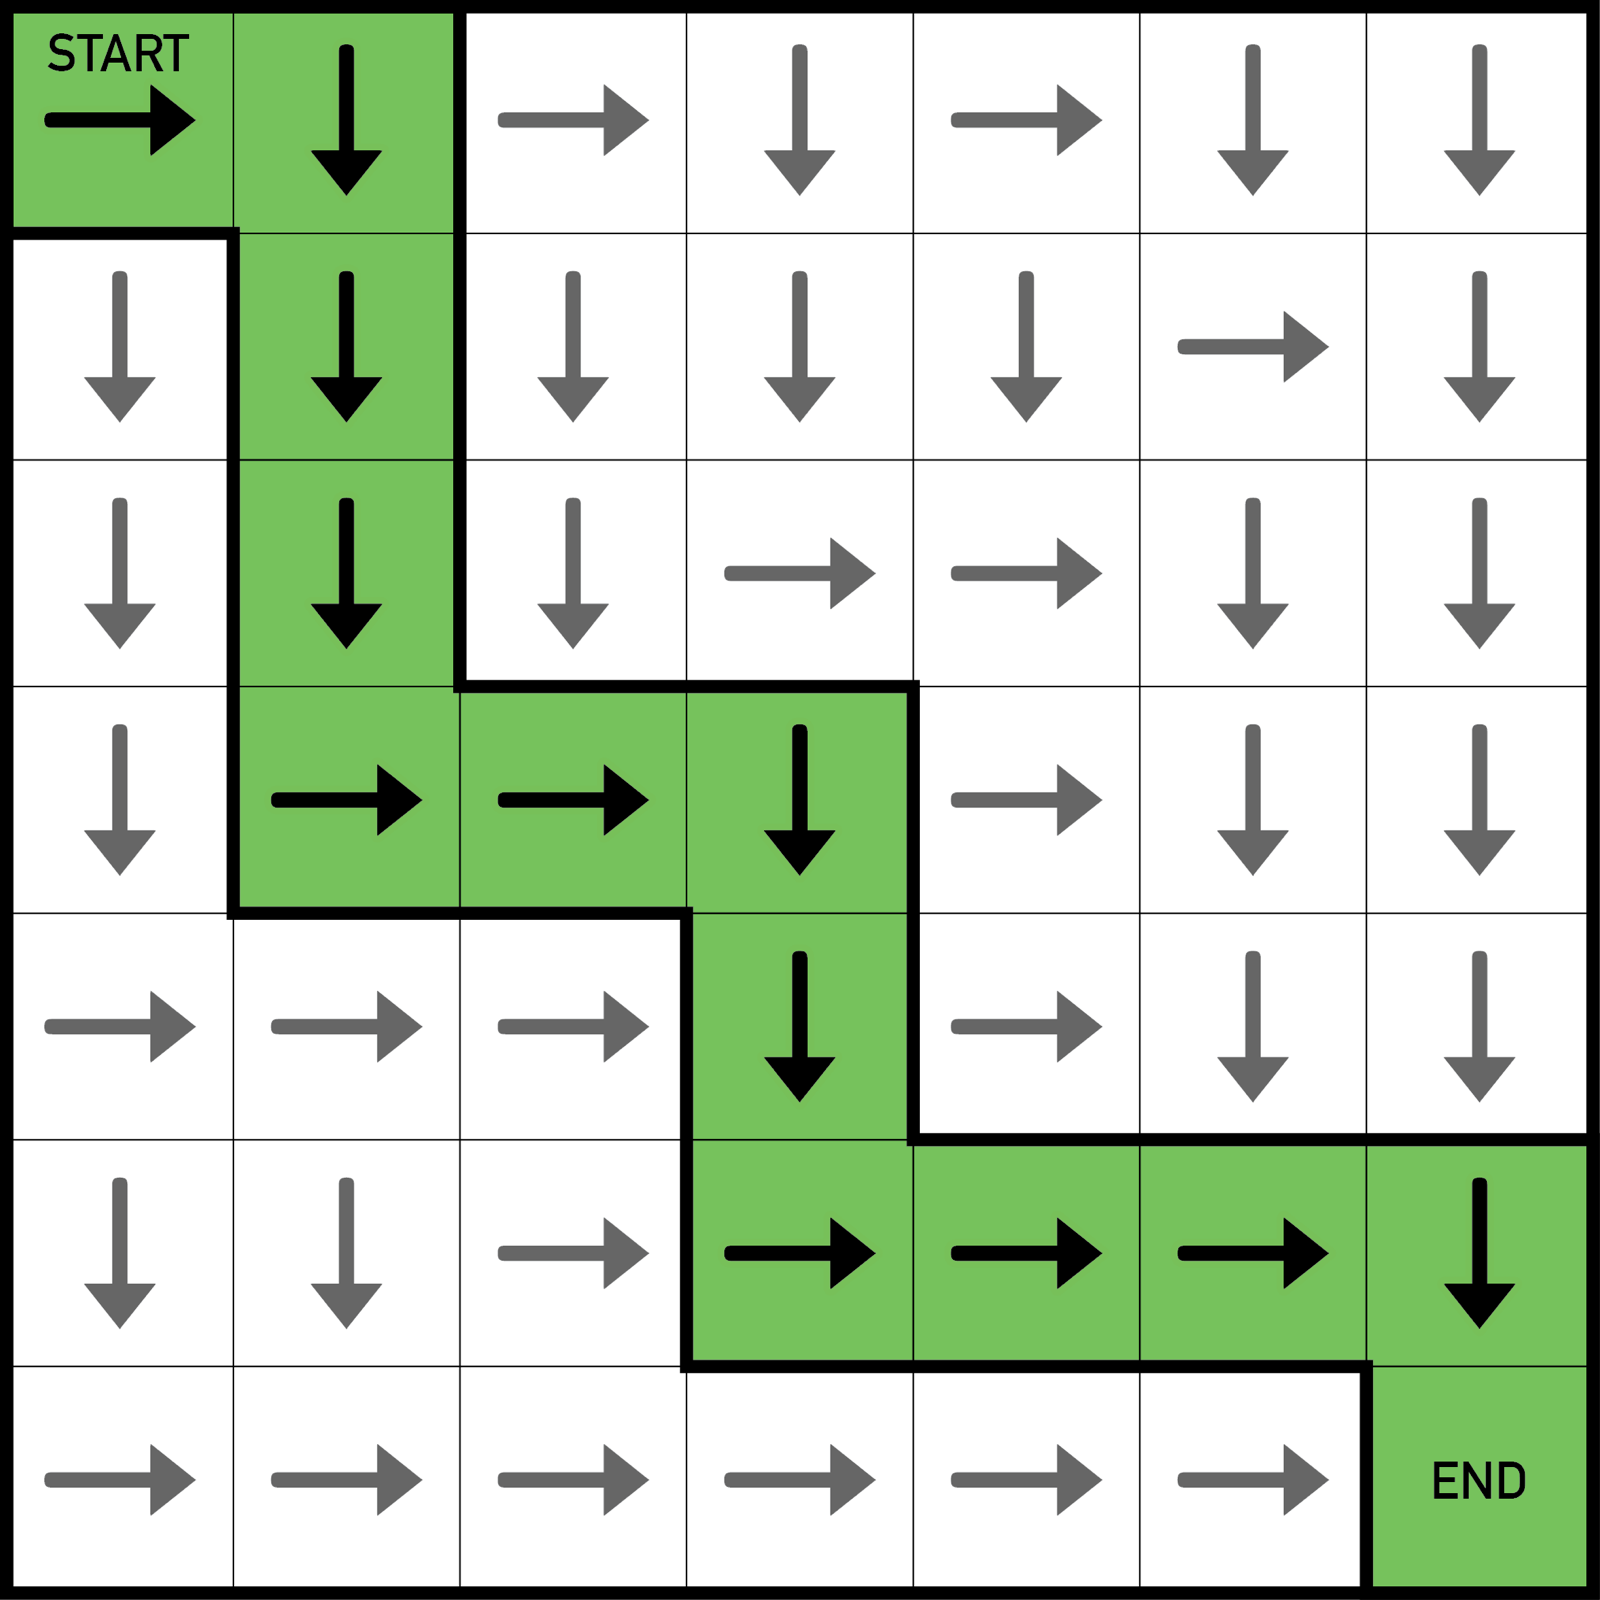
\includegraphics[width=0.2\textwidth]{figs/grid.png}
     }
     \hspace{2cm}
     \subfloat[Breakout]{%
       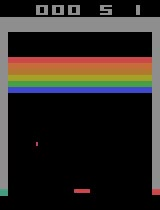
\includegraphics[width=0.15\textwidth]{figs/break.jpg}
     }
     \caption{Different RL environments}
\end{figure}
\end{frame}

%%%%%%%%%%%%%%%%%%%%%%%%%%%%%%%%%%%%%%%
\section{Motivation}
\label{sec:motivation}
\begin{frame}
  \frametitle{Motivation}
\begin{itemize}
    \item Use of Convolutional Neural Networks
    \item Input raw pixels $\xrightarrow{}$ q-function
    \item DQN algorithm (2015) $\xrightarrow{}$ Rainbow (2017)
    \item Limitations:
    \begin{itemize}
        \item Network trained separately for each task
        \item Long processing times
    \end{itemize}
    \item Possible solution $\xrightarrow{}$ Multitask and transfer RL
    \begin{itemize}
        \item Multitask - same agent solves multiple tasks
        \item Transfer - use previously acquired knowledge to facilitate learning on novel tasks
    \end{itemize}
\end{itemize}




\end{frame}

%%%%%%%%%%%%%%%%%%%%%%%%%%%%%%%%%%%%%%%%
\section{Multitask and transfer RL}
\label{sec:multi}
\begin{frame}
  \frametitle{Multitask and transfer RL on literature}
Different approaches:\\
\vspace{1cm}
\begin{itemize}
    \item \textbf{Policy distillation}: reduction of size and complexity to transfer policies from teachers to a student \cite{RusuPOLICYDISTILLATION}.
    \begin{itemize}
        \item Combine multiple policies more effectively
        \item Distilled policy: network trained to predict the same q-values given the same state.
        \item Common neural network with a specific output layer for each game
        \item Problems - inter-task q-function and reward range variance
    \end{itemize} 
\end{itemize}
 \end{frame}
 
 \begin{frame}
  \frametitle{Multitask and transfer RL on literature}
  \begin{itemize}
      \item \textbf{Distral}: policy distillation + regularization \cite{Teh2017Distral:Learning}
      \begin{itemize}
          \item Need for an expert to train the common policy 
          \item Allows for inter-teacher transfer 
          \item Policy centroid of all policies
          \item Tested on related tasks in rich 3D environments
      \end{itemize}
  \end{itemize}
  \begin{figure}
      \centering
      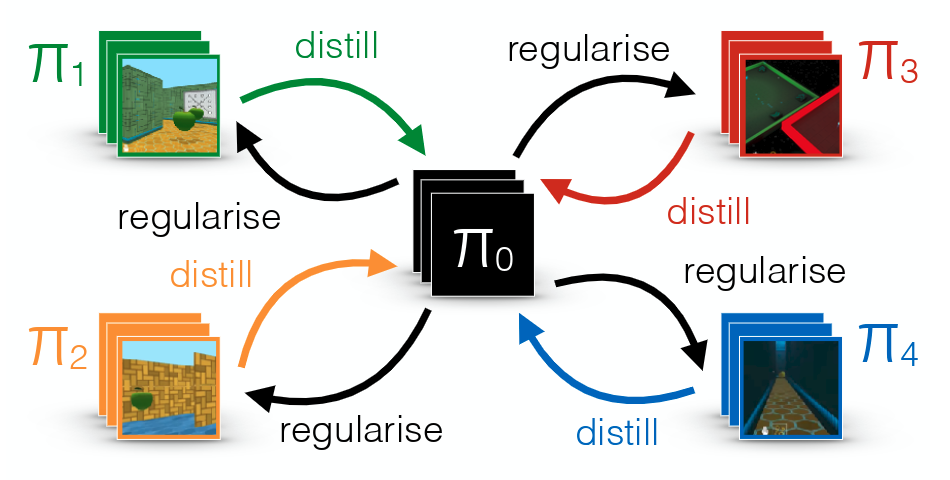
\includegraphics[scale=0.2]{figs/distral.png}
      \caption{Distral Framework}
      \label{fig:my_label}
  \end{figure}
 \end{frame}
 
\begin{frame}
  \frametitle{Multitask and transfer RL on literature}
\begin{itemize}
    \item \textbf{Actor-mimic framework}: student network that mimics experts' policies \cite{Parisotto2015Actor-Mimic:Learning}.
    \begin{itemize}
        \item Similar concept to policy distillation, but different execution.
        \item Matching expert-student q-value softmax to reduce variance
        \item Matching expert-student pre-output feature layer.
    \end{itemize} 
\end{itemize}
\begin{figure}
    \centering
    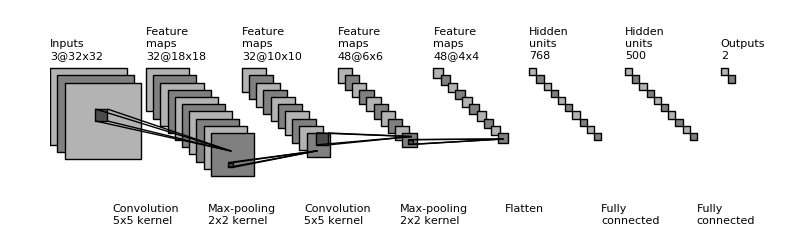
\includegraphics[scale=0.6]{figs/neural.png}
    \caption{Convolutional neural network}
    \label{fig:my_label}
\end{figure}
 \end{frame}
 
\begin{frame}
  \frametitle{Multitask and transfer RL on literature}
\begin{itemize}
    \item \textbf{New multi-task distillation architecture} + \textbf{hierarchical prioritized experience replay} \cite{YinKnowledgeReplay}
    \begin{itemize}
        \item New architecture
        \item Preventing negative transfer
        \item New sampling strategy, preserving state distribution.
    \end{itemize} 
\end{itemize}
\begin{figure}
    \centering
    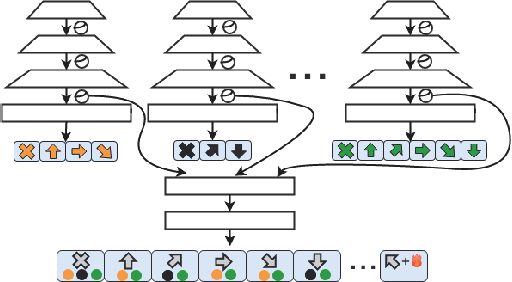
\includegraphics[scale=0.3]{figs/transfer.png}
    \caption{Proposed framework}
    \label{fig:my_label}
\end{figure}
 \end{frame}
 
\begin{frame}
  \frametitle{Multitask and transfer RL on literature} 
  \begin{figure}
      \centering
      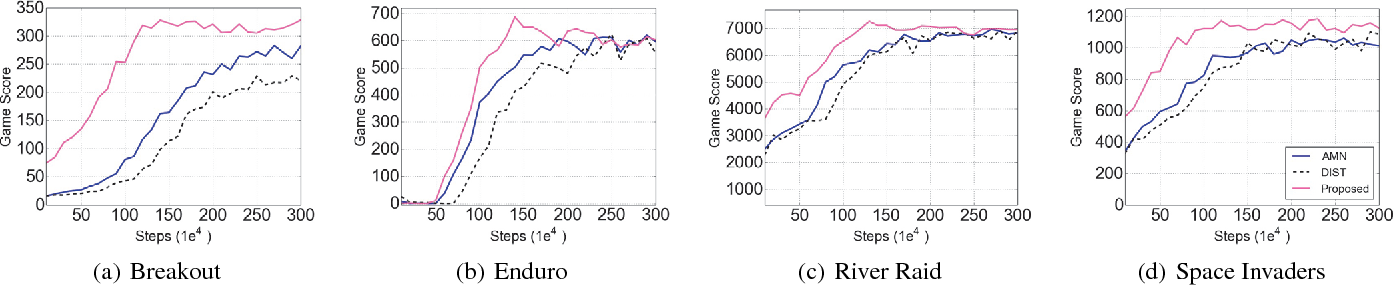
\includegraphics[scale=0.24]{figs/comparison.png}
      \caption{Benchmark of the different algorithms on Atari games.}
      \label{fig:my_label}
  \end{figure}
\end{frame}
 
\begin{frame}
\frametitle{Our algorithm}
\begin{itemize}
    \item Limitations of the existing algorithms:
    \begin{itemize}
        \item Transfer is not exploited
        \item Training times are still long
    \end{itemize}
\item Proposed algorithm:
        \begin{itemize}
            \item Not using experts
            \item Not exact same hyperparameters and smaller size
            \item Fine-tuning previous to executing a specific task
            \item Exploit similarities to favor transfer and reduce training times
        \end{itemize}
\end{itemize}
    
\end{frame}
%%%%%%%%%%%%%%%%%%%%%%%%%%%%%%%%%%%%%
\section{The continual learning problem}
\label{sec:continual}

\begin{frame}
 \frametitle{Why is catastrophic forgetting a problem?}
  \begin{itemize}
      \item Neural networks alter previous knowledge when new information is acquired.
      \item Q-values vary from task to task. Different ranges.
      \item Information needs to be consolidated without perturbing previous tasks.
  \end{itemize}
\end{frame}


\begin{frame}
 \frametitle{Continual Learning literature}
\begin{itemize}
    \item Classic solution: Interleaving new and old samples (Rehearsal)
    \item Pseudo rehearsal \cite{RobinsConsolidationBrain}
    \item Elastic Weight Consolidation \cite{Kirkpatrick2017OvercomingNetworks.}
    \item Dual-memory systems \cite{Parisi2018ContinualReview}
\end{itemize}
\begin{figure}
    \centering
    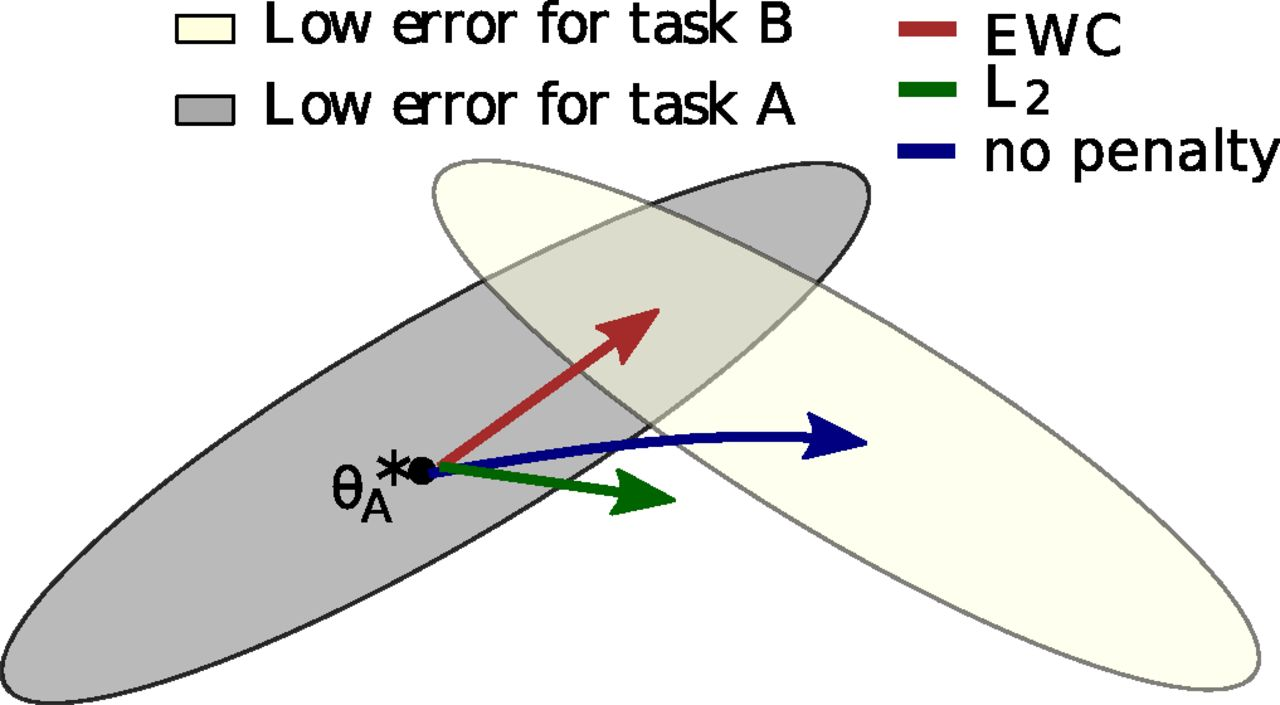
\includegraphics[scale=0.6]{figs/ewc.jpg}
    \caption{Elastic Weight Consolidation concept}
    \label{fig:my_label}
\end{figure}
  
\end{frame}


%%%%%%%%%%%%%%%%%%%%%%%%%%%%%%%%%%%%%%%%%%%
\section{Conclusion}
\label{sec:continual}
\begin{frame}
\frametitle{Conclusion}
\begin{itemize}
    \item Addressing the catastrophic forgetting problem directly gives new insight.
    \item Using pseudorehearsal and dual-memory systems as possible solutions.
    \item Our idea has been positioned in the multitask and transfer RL landscape.
\end{itemize}
\end{frame}



\begin{frame}
  \frametitle{Questions}
  \begin{center}
    Thank you for your attention.

    Do you have any questions?
  \end{center}
\end{frame}
\nobibliography{references}

\end{document}



